\chapter{Design}\label{design}

The overall design of the solution for this project mainly focused on the creation of  short 42 programs. These programs were then turned into tests that were added to the 42 automated test suite. The overall goal of the project was to discover bugs in the implementation of the 42 compiler, and a black-box testing methodology was considered to be the best way of testing the implementation. The project followed engineering and testing best-practices which helped to ensure that the outcome and deliverables of the project were as a high a standard as possible.

This chapter will cover the requirements that were set out for the project, the design of the system, process of design, and the alternative designs and approaches that were considered.

\section{Requirements Analysis \label{reqs}}

The requirements for this project were gathered from Dr. Servetto, the supervisor of this project. The initial project outline stated that ``the purpose of this project will be to write many short 42 programs trying to leverage to corner cases of the implementation and discover bugs.`` Further requirements were then gathered through discussion with Dr. Servetto during the initial planning phase of the project.

The requirements were quite wide in scope which meant there was significant freedom in how they were interpreted. The overall requirements of the project were stated as:

\begin{itemize}
	\item{Small 42 programs will be created, compiled, and then run.}
	\item{These programs will be turned into automated tests and added to the 42 test suite if they are deemed interesting.}
	\item{These programs will generally be written in a "black-box" style.}
\end{itemize}

Due to the wide scope of the project, the requirements could be considered to be somewhat vague, but they are as specific as possible for a project of this scope. This is due to the required testing of the compiler in a black-box style. The scope impacts the requirements as black-box testing does not have be a single method, and the tests do not have to focus on a specific part of the compiler. Instead the tests focus on the system as a whole. This leads to the requirements being straightforward and somewhat broad, as seen above.

\section{System Design}

\subsection{Black-box Testing \label{bbtest}}

A black-box testing methodology was the main testing methodology used over the course of this project. This methodology was chosen for two major reasons. Firstly, the outline of the project stated that  "small 42 programs will be created'', which is a goal that can only be fulfilled with a testing methodology that is at least partially of a black-box style, as the system as whole is being tested when 42 programs are created, compiled, and run.

The requirements that were gathered at the start of the project (see Section \ref{reqs}) also strongly suggested that a black-box methodology should be adopted as the requirements stated that "programs will generally be written in a black-box style".

Secondly, discussion with Dr. Servetto led to the conclusion that a black-box style of testing should be used for this project. A major reason for this was that as the time frame for this project was limited to two trimesters (approximately six months), and it was felt to be infeasible for a newcomer to the project to gain enough system knowledge to be able to test effectively test in a white-box style, and still write enough tests to make the time spent on the project worthwhile. The time spent to gain a high level of system knowledge would be likely to be a significant period of time, as like most compilers, the 42 compiler is a complex piece of software. It was felt that the time required would probably be better spent writing more tests.

Black-box testing has a significant number of techniques to choose from, and a small subset of the techniques were chosen for use in this project:

\begin{itemize} 
	\item{Use Case Testing}
	\item{Error Guessing}
	\item{Modified Orthogonal Squares}
\end{itemize}

These techniques were chosen as they provided a good blend of coverage, ease of use, and suitability for the project at hand. 

 Error guessing was chosen primarily for its value during the initial phase of the project, while the language was still being learnt. It is sometimes seen as primitive and not very useful \cite{enc2}, however it can be useful when testing compilers as many compilers have suffered from the same kinds of bugs or undefined behaviour, and error guessing allows a tester to implement lessons learned from past experiences and mistakes \cite{homes}. 

The orthogonal squares testing method used in this project was a modified version of Mandl's method \cite{Mandl} introduced in Section \ref{orthsec}. It was modified to more closely suit the project, as even with the reduction in tests required by using Mandl's method, exhaustively testing the 42 compiler would be impossible. The method was modified by limiting the \textit{k} and \textit{n} values, and therefore the size of the square, and by combining multiple test cases into one to reduce compilation times. 

Use case testing was used as it allowed for broad test coverage. This is because a scenario for a use case test of a compiler can be any program that can then be compiled. This gave flexibility to the testing regime, where if an idea for a test was thought of, it could be created and run. Use case testing is also a fairly natural way of testing a compiler, as when using a compiler a programmer will produce a program that fulfils set criteria, and use case testing allows that behaviour to be modelled.

\subsection{Grey-box Testing}

While white-box testing was rejected as the main methodology used for this project, some aspects of it were still used, primarily through the usage of grey-box testing. It was decided that some grey-box testing would be used during this project. For this project, grey-box testing was considered to be black-box testing with some system knowledge. The grey-box method chosen was use case testing, but unlike the use case testing that was used in the black-box style, system knowledge was incorporated. It was planned that grey-box testing would be used mainly to test the 42 standard library. The code for 42 standard library functions would be read, and then use case tests could be written to target specific parts of the standard library. The advantage of this method is that the level of system knowledge required would not be as high as would be required for white-box testing, but the system knowledge would still provide valuable insight. 

It was thought that these tests would be more effective than blindly trying to guess inputs that would find bugs in the 42 standard library, which would be the case if purely black-box testing was used.


\section{Testing Timeline \label{planTiming}}

As per Section \ref{bbtest} it was decided that the initial stages of the project would consist of familiarisation with 42, and error guessing testing. Error guessing was used initially as it could be used whilst learning 42. Once familiar with 42, it was decided that error guessing would be less useful and the main focus of the testing would switch to use case testing.

It was decided that the majority of testing during this project would be use case testing. This is because it is one of the more broad methods, allowing testing flexibility which was considered important when testing a compiler. The infinite input domain, which meant that exhaustive black-box testing would be impossible, was also a major factor in the choice to use a significant amount of use case testing. This meant it was planned that most of the testing time during the project would be spent doing use case testing. 

During the planning phase of the project it was unknown how effective the modified orthogonal squares method would prove to be. It was therefore decided that it would be used towards the end of the project. There were two main reasons for this. Firstly that near the end of the project, familiarity with the 42 language would be at its peak. Secondly, if the method proved to be ineffective, tests would have already been written with the other methods, and a number of bugs would (hopefully) have already been found.

\begin{figure}[h]
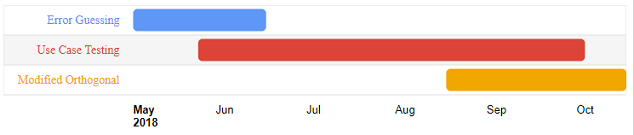
\includegraphics{nis2}
\caption{The planned time period of each testing method}
\end{figure}


\section{Alternative Approaches}

Alternative approaches to this project were considered, but for various reasons these were found to be either inadequate, inferior to the chosen approach, or not suited to the requirements of the project. When the project was initiated, it was decided that broadly scoped, manual testing would form the majority of the tests written for this project. 

While a black-box methodology was chosen for this project, a subset of testing methods had to be chosen, as some methods proved to be unsuitable for the goal of testing a compiler, and the outcomes of other styles were considered to be outweighed by the cost of implementation.
Two other major types of testing were considered, white-box testing, and a more automated testing regime.

\begin{table}
\centering
\begin{threeparttable}
 \caption{A brief comparison of the advantages and disadvantages of testing methodologies considered for this project}
    \begin{tabular}{| l | p{65mm} | p{65mm} |}
    \hline
    \textbf{Testing style} & \textbf{Pros} & \textbf{Cons} \\ \hline
    Black-box &  No knowledge of system required \newline \newline Unbiased view of codebase \newline \newline Tests are relatively uncoupled from system implementation & Practically infinite test state space \newline \newline Lack of knowledge of system may hinder efforts \newline \newline Can lead to large numbers of tests testing the exact same code\\ \hline
    White-box & Knowledge of system may help find bugs \newline \newline Test state space is smaller than black-box \newline \newline Tooling may exist to help testing &  Requires system knowledge \newline \newline Scope of testing can be extremely large \newline \newline Tests may be strongly coupled to implementation  \\ \hline
    Fuzzing & Allows the creation of many tests with little effort \newline \newline Low ongoing time cost  & High initial time cost \newline \newline Difficult to use with compilers \\ \hline
    \end{tabular}
\end{threeparttable}
\end{table}

\subsection{White-box Testing}

White-box, as presented in Section \ref{whitebox}, is a testing methodology that focuses on "test methods that rely on the internal structure of the software" \cite{ostrand}. This means that the author of the tests has to have significant knowledge of the inner workings of the system that they are testing. Major white box testing styles include structured testing \cite{watson}, branch testing, path testing, and statement coverage \cite{ammann} \cite{khan2012}. Some of these techniques could have been useful, but time constraints, the problem domain of a compiler, and the gathered requirements meant that it was felt that a different methodology, namely black-box, would produce better results for this project. 

\subsubsection{Advantages}

One of the main advantages of a white-box testing methodology in regards to this project is that a tester is required to have a good knowledge of the system. This means that the tester may have a good idea of where bugs could be found in the system, as they understand the code, and should therefore understand where testing effort would best be applied. This could be useful in a compiler as knowledge of how the system works at a low level could be helpful in locating bugs.

White-box testing is said to be easy to automate \cite{ammann}, which can be a major advantage, especially when testing a large scale project such as a compiler. Many automated tests could be produced that could provide fairly high branch and statement coverage. 

If statement or branch coverage testing were to be used in a white-box methodology, a clear idea of how "tested" the program is, could be determined. This level of "testedness" could be found by using a simple code coverage tool which would list the percentage of statements and branches covered by unit tests. 

\subsubsection{Disadvantages}

One of the main disadvantages of white-box testing is that a high level of system knowledge is required. This means that before starting testing, the tester will have to spend time familiarising themselves with the system instead of testing. This is especially true in the case of testing a system as complex as a compiler. System knowledge for this project would be difficult to gain in a timely manner, due to the fact that the 42 compiler is a complex system.

Another reason for not using a white-box methodology for this project was that the initial idea of the project is that the compiler would be tested as a whole by creating 42 programs and attempting to run them. There was discussion about the possibility of white-box testing but Dr. Servetto felt it would not be the best path for this project, as it was felt that black-box testing of the system as a whole would be more effective.

Another major problem with white-box testing in terms of this project is that a compiler has a practically infinite input domain. This means that any white-box testing will struggle to fulfil the ideal case of being exhaustive (see Section \ref{whitebox}). White-box testing makes exhaustive unit testing very difficult, especially in regards to path coverage. Due to the extremely large numbers of possible paths, it would be very difficult for path testing to provide any semblance of exhaustiveness in terms of test coverage.

\subsection{Fuzz Testing}

Fuzzing consists of generating random data, called fuzz and using it as input into a program. In the case a of compiler, it would generally consist of generating random programs that could then be attempted to be compiled and run. A prototype, very simple fuzzer, focused on 42 was developed (see the TestIncrementer section below) for this project. It proved to be not very useful, and showed that a "dumb" fuzzer would not be very useful for this project.

Overall it was decided to not pursue fuzzing for this project as existing tools would not have worked very well on the 42 compiler. Specially created "dumb" tools proved they would not be very useful, and a "smart" tool would have taken far too long to create, and would have been significantly out of scope for this project.

\subsubsection{Advantages}

Fuzzing is highly automated once set up, therefore once a fuzzer is initially set up, very little user input would be required, except in the case of dealing with a potential bug the fuzzer has found.

Additionally, due to the fact that fuzzing can be highly automated, fuzzing would produce far more tests than could reasonably be produced manually. If these tests actually managed to test the 42 compiler as a whole (by being syntactically correct 42 programs), fuzzing would be a major help for this project.

\subsubsection{Disadvantages}

Fuzz testing cannot provide a complete picture of the entirety of the program, especially in the case of a compiler. This is because generating random data to test a compiler would probably take the form of generating random strings and trying to compile them as programs. These strings, if randomly generated, are extremely unlikely to be syntactically correct enough to compile, let alone test any interesting behaviour of the 42 language.

Another issue with using fuzzing in this project would be the sourcing of a suitable fuzzer. Most fuzzers are designed to work on C code \cite{afl}. The 42 compiler is coded in Java, and while there are Java fuzzers, they are less advanced and not as effective.

The most effective fuzzer for this project would one that is "smart" enough to be aware of the input structure a file that could be compiled by the 42 compiler. This would probably take the form of a fuzzer that could produce syntactically correct 42 code as an output, and this code could be run and then manually checked if there were some sort of anomaly or error. The creation of this kind of fuzzer would require a significant amount of work, if it is even possible.

\subsubsection{Test Incrementer \label{incrementerSec}}
The 42TestIncrementer \cite{incrementer} is a Python "dumb" fuzzer specifically created for this project. It creates 42 programs by very slightly modifying existing 42 programs. It can be given a .L42 (42's file extension) file, and it will search that file for method declarations. From the given set of method declarations, the incrementer will check through all methods to check if a method takes \textit{Num} (42's arbitrary-precision number class) or an \textit{S} (42's string class) as a method parameter. If a method takes a \textit{Num} or an \textit{S}, the incrementer will modify the parameter in the method call. This modification can either be by set value or random value depending on the way the flags passed to the incrementer.

This program is not particularly advanced, and will only work for method calls that directly have a \textit{Num} or \textit{S} declared in method call. The incrementer had some problems, as there was relatively little time spent developing it, as it was more a proof of concept as opposed to a final polished product. This meant that it is fairly limited; it only works for \textit{Num} and \textit{S} types and does not handle recursion or method overriding very well. It is possible that more time could have been spent on developing the tool, but any more time spent on developing the incrementer would be time that would have had to have been taken away from direct test creation.

The incrementer was a proof of concept and it proved that a "dumb" fuzzer would not be very useful for this project. 42 has arbitrary-precision numbers therefore number overflow was not a risk, and this was the main type of error that the incrementer would have found.

For an example of the 42TestIncrementer see Appendix \ref{incrementerExample} where it is used to slightly modify a program.



